%\documentclass[12pt a4papel]{article}
\documentclass[12pt]{article}
\usepackage[utf8]{inputenc}
\usepackage{lipsum}
\usepackage{xcolor}
\usepackage{graphicx}

\title{HIPOTESIS DEL BOSQUE OSCURO}
\author{Tatiana}
\date{3 de abril 2024}
\begin{document}
\tableofcontents
\maketitle
\noindent
este es el indice del articulo
\section{INDICE}
\subsection{Introducción}
\lipsum[1-2]
\subsection{¿Porque no es tan fácil encontrar esta vida inteligente?}
\lipsum[1]
\section{tablas}
\begin{center}
\begin{tabular}{|c|c|c|}
\hline
\multicolumn{3}{c}{lista de nombres}\\
\hline
\hline
\color{red}
\bf nro & \color{red}\bf nombre & \color{red}\bf movil \\
   \hline
    1  &  Juan  & 7140914\\
    \hline
    2  &  Pedro & 4148785\\
    \hline
\end{tabular}
\end{center}
\section{graficos}
\begin{figure}
    \centering
    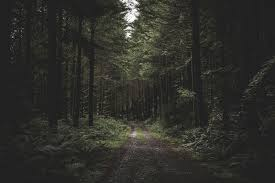
\includegraphics[width=0.45\linewidth]{bosqueblack.jpeg}
    \caption{\label{bosqueblack.jpeg}this bosque was uploaded via the file-tree menu.}{Bosque oscuro}
    \label{fig:enter-label}
\end{figure}
\subsection{Hipotesis del bosque oscuro}
\lipsum[1-5]
\subsection{Explicación de la paradoja de Fermi}
\lipsum[1-2]
\subsection{SETI}
\lipsum[1-2]
\subsection{METI}
\lipsum[1-2]
\subsection{Existen dos escenarios posibles de :}
\lipsum[1-3]
\end{document}